\documentclass{beamer}
\usetheme{CambridgeUS}
\usepackage{tikz}
\usetikzlibrary{matrix,arrows,fit,positioning, mindmap, trees}

\usepackage[latin1]{inputenc}
\usefonttheme{professionalfonts}
\usepackage{times}
\usepackage{xmpmulti}
\usepackage{animate}
\usepackage{amsmath}
\usepackage{verbatim}
\usepackage{graphicx}
\usepackage{xcolor}
\usepackage{mathrsfs}  
\usepackage{bussproofs}
\usepackage{tikz}
\usetikzlibrary{shapes.geometric, positioning}
\graphicspath{ {./images/} }
%\usetheme{Boadilla}
%\usecolortheme{crane}
\title[Formal Verification]{Formal verification of systems -- a survey of approaches from classical to recent developments}
%\subtitle{I Am Curious}
\author[Sebastian Schlesinger]{Prof. Dr.-Ing. Sebastian Schlesinger}
\institute[HWR Berlin]{Berlin School for Economics and Law}
\date{\today}
\begin{document}
 \begin{frame}
\titlepage
\end{frame}
\begin{frame}
\frametitle{Objectives}
\begin{itemize}
\item Obtain an initial understanding of formal concepts
\item Survey of classical and recent approaches to formal verification
\item Also establish the bridge to related work and future research directions I am aiming at
 
\end{itemize}

\end{frame}
\begin{frame}{My Research Focus}
  My background: \textbf{formal verification} (particularly model-driven engineering of embedded or cyber-physical systems) and \textbf{security}. 
  Recently, also \textbf{machine learning}. 

  So, in essence, I am interested in \textbf{safety} and \textbf{security} of \textbf{AI-enabled systems} or the application of \textbf{Machine Learning} to classical approaches for the verification of safety and security of systems.
  \begin{center}
  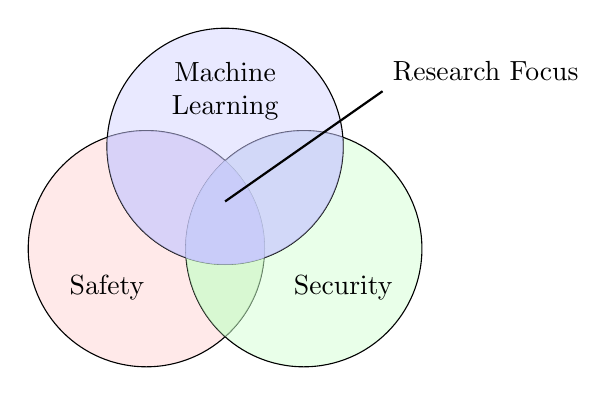
\begin{tikzpicture}
    % Colors with opacity
    \definecolor{color1}{RGB}{255, 200, 200}
    \definecolor{color2}{RGB}{200, 255, 200}
    \definecolor{color3}{RGB}{200, 200, 255}
    
    % Circles
    \draw[fill=color1, fill opacity=0.4] (0,0) circle (1.5cm);
    \draw[fill=color2, fill opacity=0.4] (2,0) circle (1.5cm);
    \draw[fill=color3, fill opacity=0.4] (1, 1.3) circle (1.5cm);
    
    % Darker intersections
    \begin{scope}
      \clip (0,0) circle (1.5cm);
      \fill[color2, opacity=0.5] (2,0) circle (1.5cm);
    \end{scope}
    
    \begin{scope}
      \clip (0,0) circle (1.5cm);
      \fill[color3, opacity=0.5] (1,1.3) circle (1.5cm);
    \end{scope}
    
    \begin{scope}
      \clip (2,0) circle (1.5cm);
      \fill[color3, opacity=0.5] (1,1.3) circle (1.5cm);
    \end{scope}
    
    \begin{scope}
      \clip (0,0) circle (1.5cm);
      \clip (2,0) circle (1.5cm);
      \fill[color3, opacity=0.5] (1,1.3) circle (1.5cm);
    \end{scope}
  
    % Annotations within the circles
    \node at (-0.5, -0.5) {Safety};
    \node at (2.5, -0.5) {Security};
    \node at (1, 2) {\begin{tabular}{c} Machine \\ Learning \end{tabular}};
    
    % Line pointing to "Research Focus"
  \draw[-, thick] (1, 0.6) -- (3, 2) node[above right] {Research Focus};
  
  \end{tikzpicture}
  \end{center}
\end{frame}


\begin{frame}
  \frametitle{Outline}
  \tableofcontents
\end{frame}

\section{Introduction}


\begin{frame}
  \frametitle{Embedded Systems}
  
  \begin{center}
    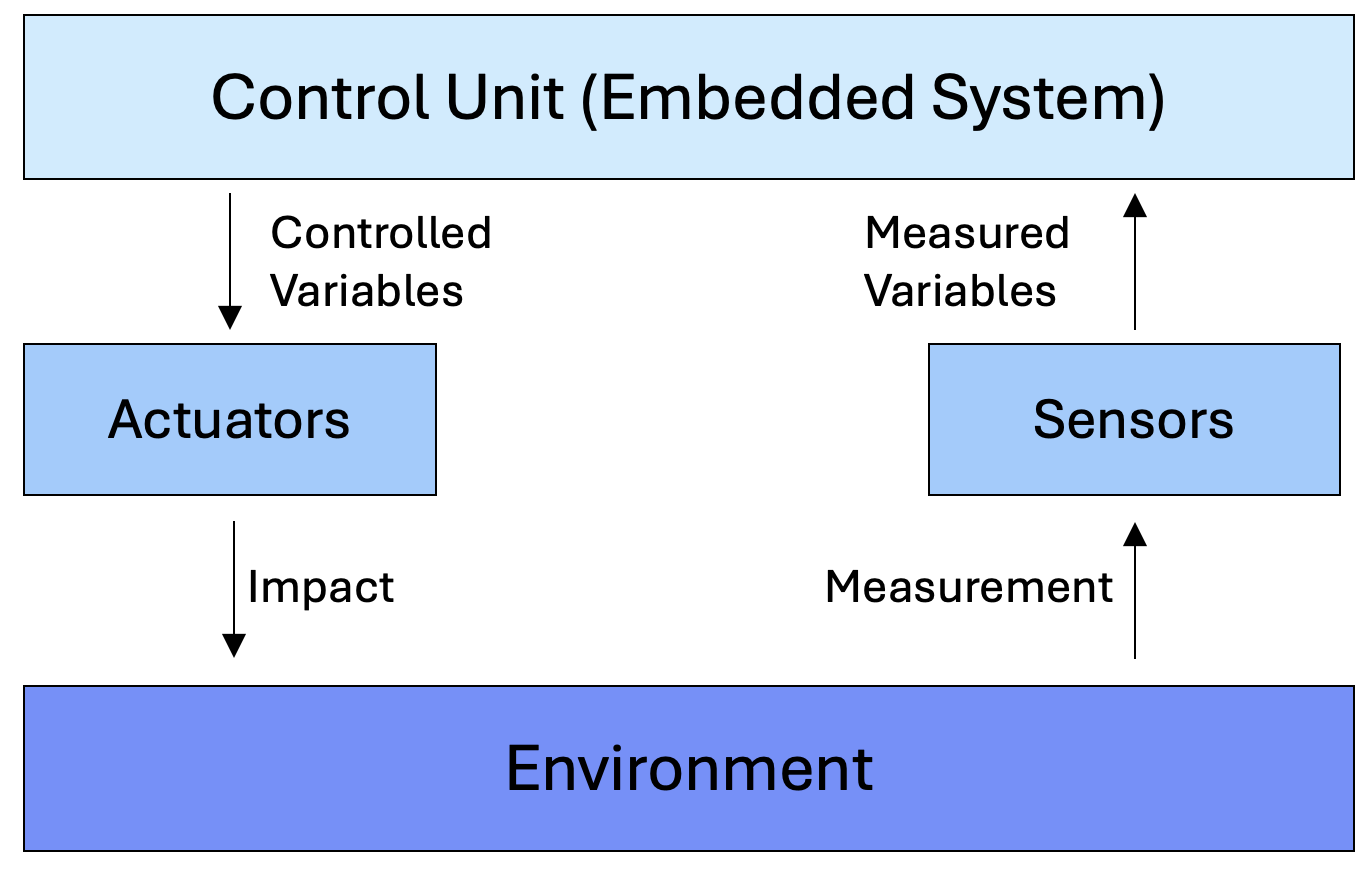
\includegraphics[width=\linewidth]{images/embedded_system.png}
  \end{center}
  
  \end{frame}

  \begin{frame}{Why formal verification?}
  
  \end{frame}

\section{First-order logic}
\begin{frame}{Language of first-order logic}
  
    A language $\mathscr{L}$ of first-order logic consists of the following components:
    \begin{itemize}
    \item Variable symbols: $x_1, x_2, \ldots$
    \item For each $n\in\mathbb{N}$, a set of $n$-ary function symbols: $f_0, f_1, \ldots$ The 0-ary function symbols are called constant symbols.
    \item For each $n\in\mathbb{N}$, a set of $n$-ary predicate symbols: $p_0, p_1, \ldots$ The 0-ary predicate symbols are the constants $\top$ (for \textbf{true}) and $\bot$ (for \textbf{false}).
    \item special symbols: $\neg$ (negation), $\wedge$ (conjunction), $\vee$ (disjunction), $\rightarrow$ (implication), $\leftrightarrow$ (equivalence), $\forall$ (universal quantification), $\exists$ (existential quantification), and parentheses.
  \end{itemize}

  \end{frame}

  \begin{frame}{Terms}

    The set of terms of $\mathscr{L}$ is defined inductively as follows:
    \begin{itemize}
    \item Each variable is a term.
    \item If $t_1, \ldots, t_n$ are terms and $f$ is an $n$-ary function symbol, then if $f(t_1, \ldots, t_n)$ is a term.
  \end{itemize}
  \end{frame}

  \begin{frame}{Variables in terms}
    We define a function $var: \text{Terms}\rightarrow\text{Variables}$ that maps each term to the set of variables occurring in it. The function is defined as follows:
    \begin{itemize}
    \item $var(x) = \{x\}$ for each variable $x$.
    \item $var(f(t_1, \ldots, t_n)) = var(t_1)\cup\ldots\cup var(t_n)$.
  \end{itemize}
  \end{frame}
  \begin{frame}{Formulas}
    The set of formulas of $\mathscr{L}$ is defined inductively as follows:
    \begin{itemize}
    \item If $t_1, \ldots, t_n$ are terms and $p$ is an $n$-ary predicate symbol, then if $p(t_1, \ldots, t_n)$ is a formula.
    \item If $\varphi$ is a formula, then if $\neg\varphi$ is a formula.
    \item If $\varphi_1$ and $\varphi_2$ are formulas, then if $\varphi_1\wedge\varphi_2$, $\varphi_1\vee\varphi_2$, $\varphi_1\rightarrow\varphi_2$, and $\varphi_1\leftrightarrow\varphi_2$ are formulas.
    \item If $\varphi$ is a formula and $x$ is a variable, then if $\forall x.\varphi$ and $\exists x.\varphi$ are formulas.
  \end{itemize}
  An example of a formula is $\forall x. \exists y. p(x, y) \rightarrow \neg q(y)$.
  \end{frame}

  \begin{frame}{Interpretations}
    
    An interpretation $\mathcal{M}$ of $\mathscr{L}$ consists of the following components:
    \begin{itemize}
    \item A non-empty set $D$ called the domain of $\mathcal{M}$.
    \item For each $n$-ary function symbol $f$ of $\mathscr{L}$, a function $f^{\mathcal{M}}: D^n\rightarrow D$.
    \item For each $n$-ary predicate symbol $p$ of $\mathscr{L}$, a relation $p^{\mathcal{M}}\subseteq D^n$.
  \end{itemize}
  \end{frame}

  \begin{frame}{Interpretations of Terms}
    Let $\mathcal{M}$ be an interpretation for our first-order language. 
    An assignment $\sigma$ of values to variables, i.e., $\sigma: Variables\rightarrow D$. 
    
    The value of a term $t$ under $\sigma$ is denoted by $t^{\mathcal{M}}[\sigma]$ and defined as follows:
    \begin{itemize}
    \item If $t=x$ for a variable $x$, then $t^{\mathcal{M}}[\sigma]=\sigma(x)$.
    \item If $t=f(t_1, \ldots, t_n)$, then $t^{\mathcal{M}}[\sigma]=f^{\mathcal{M}}(t_1^{\mathcal{M}}[\sigma], \ldots, t_n^{\mathcal{M}}[\sigma])$.
    \end{itemize}
  \end{frame}
  \begin{frame}{Validity of Formulas under Interpretations}
    We say an assignment $\sigma$ satisfies a formula $\varphi$ under an interpretation $\mathcal{M}$, denoted by $\mathcal{M}, \sigma\models\varphi$, iff the following conditions hold:
    \begin{itemize}
    \item $\varphi=p(t_1, \ldots, t_n)$, then if $(t_1^{\mathcal{M}}[\sigma], \ldots, t_n^{\mathcal{M}}[\sigma])\in p^{\mathcal{M}}$.
    \item $\varphi=\neg\psi$, then if $\mathcal{M}, \sigma\not\models\psi$.
    \item $\varphi=\psi_1\vee\psi_2$, then if $\mathcal{M}, \sigma\models\psi_1$ or $\mathcal{M}, \sigma\models\psi_2$.
    \item $\varphi=\psi_1\wedge\psi_2$, then if $\mathcal{M}, \sigma\models\psi_1$ and $\mathcal{M}, \sigma\models\psi_2$.
    \item $\varphi=\psi_1\rightarrow\psi_2$, then if $\mathcal{M}, \sigma\models\psi_1$ implies $\mathcal{M}, \sigma\models\psi_2$.
    \item $\varphi=\psi_1\leftrightarrow\psi_2$, then if $\mathcal{M}, \sigma\models\psi_1$ if and only if $\mathcal{M}, \sigma\models\psi_2$.
    \item $\varphi=\forall x.\psi$, then if $\mathcal{M}, \sigma[x\mapsto d]\models\psi$ for all $d\in D$.
    \item $\varphi=\exists x.\psi$, then if $\mathcal{M}, \sigma[x\mapsto d]\models\psi$ for some $d\in D$.
    \end{itemize}
    A formula $\varphi$ is satisfiable if there exists an interpretation $\mathcal{M}$ and an assignment $\sigma$ such that $\mathcal{M}, \sigma\models\varphi$.
  \end{frame}


  \begin{frame}{Models}
    An interpretation $\mathcal{M}$ is a model of a formula $\varphi$, denoted by $\mathcal{M}\models\varphi$, if for all assignments $\sigma$, $\mathcal{M}, \sigma\models\varphi$.
    
    
    
  \end{frame}
 

  \begin{frame}{Validity}
    A formula $\varphi$ is valid if for all interpretations $\mathcal{M}$ and all assignments $\sigma$, $\mathcal{M}, \sigma\models\varphi$.
    
    We write $\models\varphi$ to denote that $\varphi$ is valid.
  \end{frame}

  \begin{frame}{Free Variables in Fomulas}
    The set of free variables of a formula $\varphi$, denoted by $FV(\varphi)$, is defined inductively as follows:
    \begin{itemize}
    \item $FV(p(t_1, \ldots, t_n))=var(t_1)\cup\ldots\cup var(t_n)$.
    \item $FV(\neg\psi)=FV(\psi)$.
    \item $FV(\psi_1\wedge\psi_2)=FV(\psi_1)\cup FV(\psi_2)$.
    \item $FV(\psi_1\vee\psi_2)=FV(\psi_1)\cup FV(\psi_2)$.
    \item $FV(\psi_1\rightarrow\psi_2)=FV(\psi_1)\cup FV(\psi_2)$.
    \item $FV(\forall x.\psi)=FV(\psi)\setminus\{x\}$.
    \item $FV(\exists x.\psi)=FV(\psi)\setminus\{x\}$.
    \end{itemize}
  \end{frame}

  \begin{frame}{Term Substitution}
    Let $\varphi$ be a formula, $x$ a variable, and $t$ a term. The formula $\varphi[x\mapsto t]$ is obtained by replacing all occurrences of $x$ in $\varphi$ by $t$. The substitution is defined inductively as follows:
    \begin{itemize}
    \item $(p(t_1, \ldots, t_n))[x\mapsto t]=p(t_1[x\mapsto t], \ldots, t_n[x\mapsto t])$.
    \item $(\neg\psi)[x\mapsto t]=\neg\psi[x\mapsto t]$.
    \item $(\psi_1\wedge\psi_2)[x\mapsto t]=\psi_1[x\mapsto t]\wedge\psi_2[x\mapsto t]$.
    \item $(\psi_1\vee\psi_2)[x\mapsto t]=\psi_1[x\mapsto t]\vee\psi_2[x\mapsto t]$.
    \item $(\psi_1\rightarrow\psi_2)[x\mapsto t]=\psi_1[x\mapsto t]\rightarrow\psi_2[x\mapsto t]$.
    \item   $(\forall y.\psi)[x\mapsto t]=\forall y.\psi[x\mapsto t]$ if $x\in FV(t)$.
    \item $(\exists y.\psi)[x\mapsto t]=\exists y.\psi[x\mapsto t]$ if $x\in FV(t)$.
    \item $(\forall x.\psi)[x\mapsto t]=\forall x.\psi$.
    \item $(\exists x.\psi)[x\mapsto t]=\exists x.\psi$.
    \end{itemize}
  \end{frame}
    
  \begin{frame}{Calculus}
    A calculus is a mechanism to prove formulas by applying rules.

    A rule of a calculus has the form $\frac{\varphi_1, \ldots, \varphi_n}{\psi}$, where $\varphi_1, \ldots, \varphi_n$ are premises and $\psi$ is the conclusion. The rule states that if $\varphi_1, \ldots, \varphi_n$ are derivable, then $\psi$ is derivable.

    We denote that a formula can be proved by a calculus by $\vdash\varphi$.
  \end{frame}
% ****************************



\begin{frame}
  \frametitle{Natural Deduction Rules}
  \begin{columns}
  
  \column{0.5\textwidth}
  \textbf{Conjunction Introduction ($\land$ I)}
  \begin{prooftree}
    \AxiomC{$A$}
    \AxiomC{$B$}
    \RightLabel{$\land$ I}
    \BinaryInfC{$A \land B$}
  \end{prooftree}
  
  \vspace{10pt}
  
  \textbf{Conjunction Elimination ($\land$ E)}
  \begin{prooftree}
    \AxiomC{$A \land B$}
    \RightLabel{$\land$ E$_1$}
    \UnaryInfC{$A$}
  \end{prooftree}
  \begin{prooftree}
    \AxiomC{$A \land B$}
    \RightLabel{$\land$ E$_2$}
    \UnaryInfC{$B$}
  \end{prooftree}
  
  \column{0.5\textwidth}
  \textbf{Disjunction Introduction ($\lor$ I)}
  \begin{prooftree}
    \AxiomC{$A$}
    \RightLabel{$\lor$ I$_1$}
    \UnaryInfC{$A \lor B$}
  \end{prooftree}
  \begin{prooftree}
    \AxiomC{$B$}
    \RightLabel{$\lor$ I$_2$}
    \UnaryInfC{$A \lor B$}
  \end{prooftree}
  
  \vspace{10pt}
  
  \textbf{Disjunction Elimination ($\lor$ E)}
  \begin{prooftree}
    \AxiomC{$A \lor B$}
    \AxiomC{$[A]$}
    \noLine
    \UnaryInfC{$\vdots$}
    \noLine
    \UnaryInfC{$C$}
    \AxiomC{$[B]$}
    \noLine
    \UnaryInfC{$\vdots$}
    \noLine
    \UnaryInfC{$C$}
    \RightLabel{$\lor$ E}
    \TrinaryInfC{$C$}
  \end{prooftree}
  
  \end{columns}
  \end{frame}
  
  \begin{frame}
  \frametitle{Natural Deduction Rules (cont.)}
  \begin{columns}
  
  \column{0.5\textwidth}
  \textbf{Implication Introduction ($\implies$ I)}
  \begin{prooftree}
    \AxiomC{$[A]$}
    \noLine
    \UnaryInfC{$\vdots$}
    \noLine
    \UnaryInfC{$B$}
    \RightLabel{$\implies$ I}
    \UnaryInfC{$A \implies B$}
  \end{prooftree}
  
  \vspace{10pt}
  
  \textbf{Implication Elimination (Modus Ponens, $\implies$ E)}
  \begin{prooftree}
    \AxiomC{$A \implies B$}
    \AxiomC{$A$}
    \RightLabel{$\implies$ E}
    \BinaryInfC{$B$}
  \end{prooftree}
  
  \column{0.5\textwidth}
  \textbf{Negation Introduction ($\neg$ I)}
  \begin{prooftree}
    \AxiomC{$[A]$}
    \noLine
    \UnaryInfC{$\vdots$}
    \noLine
    \UnaryInfC{$\bot$}
    \RightLabel{$\neg$ I}
    \UnaryInfC{$\neg A$}
  \end{prooftree}
  
  \vspace{10pt}
  
  \textbf{Negation Elimination ($\neg$ E)}
  \begin{prooftree}
    \AxiomC{$A$}
    \AxiomC{$\neg A$}
    \RightLabel{$\neg$ E}
    \BinaryInfC{$\bot$}
  \end{prooftree}
  
  \end{columns}
  \end{frame}
  
  \begin{frame}
  \frametitle{Natural Deduction Rules (cont.)}
  \begin{columns}
  
  \column{0.5\textwidth}
  \textbf{Double Negation Elimination ($\neg\neg$ E)}
  \begin{prooftree}
    \AxiomC{$\neg\neg A$}
    \RightLabel{$\neg\neg$ E}
    \UnaryInfC{$A$}
  \end{prooftree}
  
  \vspace{10pt}
  
  \textbf{Biconditional Introduction ($\iff$ I)}
  \begin{prooftree}
    \AxiomC{$A \implies B$}
    \AxiomC{$B \implies A$}
    \RightLabel{$\iff$ I}
    \BinaryInfC{$A \iff B$}
  \end{prooftree}
  
  \column{0.5\textwidth}
  \textbf{Biconditional Elimination ($\iff$ E)}
  \begin{prooftree}
    \AxiomC{$A \iff B$}
    \RightLabel{$\iff$ E$_1$}
    \UnaryInfC{$A \implies B$}
  \end{prooftree}
  \begin{prooftree}
    \AxiomC{$A \iff B$}
    \RightLabel{$\iff$ E$_2$}
    \UnaryInfC{$B \implies A$}
  \end{prooftree}
  
  \end{columns}
  \end{frame}

  \begin{frame}
    \frametitle{Natural Deduction Rules: Quantifiers}
    \begin{columns}
    
    \column{0.5\textwidth}
    \textbf{Universal Introduction ($\forall$ I)}
    \begin{prooftree}
      \AxiomC{$[x]$}
      \noLine
      \UnaryInfC{$\vdots$}
      \noLine
      \UnaryInfC{$A(x)$}
      \RightLabel{$\forall$ I}
      \UnaryInfC{$\forall x \, A(x)$}
    \end{prooftree}
    
    \vspace{10pt}
    
    \textbf{Universal Elimination ($\forall$ E)}
    \begin{prooftree}
      \AxiomC{$\forall x \, A(x)$}
      \RightLabel{$\forall$ E}
      \UnaryInfC{$A(t)$}
    \end{prooftree}
    
    \column{0.5\textwidth}
    \textbf{Existential Introduction ($\exists$ I)}
    \begin{prooftree}
      \AxiomC{$A(t)$}
      \RightLabel{$\exists$ I}
      \UnaryInfC{$\exists x \, A(x)$}
    \end{prooftree}
    
    \vspace{10pt}
    
    \textbf{Existential Elimination ($\exists$ E)}
    \begin{prooftree}
      \AxiomC{$\exists x \, A(x)$}
      \AxiomC{$[A(x)]$}
      \noLine
      \UnaryInfC{$\vdots$}
      \noLine
      \UnaryInfC{$C$}
      \RightLabel{$\exists$ E}
      \BinaryInfC{$C$}
    \end{prooftree}
    
    \end{columns}
    \end{frame}

    \begin{frame}
      \frametitle{Example Deduction: \(\forall x (P(x) \rightarrow Q(x)), \forall x P(x) \vdash \forall x Q(x)\)}
      
      \begin{prooftree}
        \AxiomC{}
        \RightLabel{Premise}
        \UnaryInfC{$\forall x (P(x) \rightarrow Q(x))$}
        \AxiomC{}
        \RightLabel{Premise}
        \UnaryInfC{$\forall x P(x)$}
        \RightLabel{$\forall$ E}
        \UnaryInfC{$P(a)$}
        \RightLabel{$\forall$ E}
        \UnaryInfC{$P(a) \rightarrow Q(a)$}
        \RightLabel{$\rightarrow$ E}
        \BinaryInfC{$Q(a)$}
        \RightLabel{$\forall$ I}
        \UnaryInfC{$\forall x Q(x)$}
      \end{prooftree}
      
      \end{frame}
%*****************
    \begin{frame}
      \frametitle{Sequent Calculus Rules: Logical Connectives}
      \begin{columns}
      
      \column{0.5\textwidth}
      \textbf{Conjunction Rules ($\land$)}
      \begin{prooftree}
        \AxiomC{$\Gamma \vdash A$}
        \AxiomC{$\Gamma \vdash B$}
        \RightLabel{$\land$ R}
        \BinaryInfC{$\Gamma \vdash A \land B$}
      \end{prooftree}
      
      \begin{prooftree}
        \AxiomC{$\Gamma, A \land B \vdash \Delta$}
        \RightLabel{$\land$ L$_1$}
        \UnaryInfC{$\Gamma, A \vdash \Delta$}
      \end{prooftree}
      \begin{prooftree}
        \AxiomC{$\Gamma, A \land B \vdash \Delta$}
        \RightLabel{$\land$ L$_2$}
        \UnaryInfC{$\Gamma, B \vdash \Delta$}
      \end{prooftree}
      
      \column{0.5\textwidth}
      \textbf{Disjunction Rules ($\lor$)}
      \begin{prooftree}
        \AxiomC{$\Gamma \vdash A$}
        \RightLabel{$\lor$ R$_1$}
        \UnaryInfC{$\Gamma \vdash A \lor B$}
      \end{prooftree}
      \begin{prooftree}
        \AxiomC{$\Gamma \vdash B$}
        \RightLabel{$\lor$ R$_2$}
        \UnaryInfC{$\Gamma \vdash A \lor B$}
      \end{prooftree}
      
      \begin{prooftree}
        \AxiomC{$\Gamma, A \vdash \Delta$}
        \AxiomC{$\Gamma, B \vdash \Delta$}
        \RightLabel{$\lor$ L}
        \BinaryInfC{$\Gamma, A \lor B \vdash \Delta$}
      \end{prooftree}
      
      \end{columns}
      \end{frame}
      
      \begin{frame}
      \frametitle{Sequent Calculus Rules: Logical Connectives (cont.)}
      \begin{columns}
      
      \column{0.5\textwidth}
      \textbf{Implication Rules ($\implies$)}
      \begin{prooftree}
        \AxiomC{$\Gamma, A \vdash B$}
        \RightLabel{$\implies$ R}
        \UnaryInfC{$\Gamma \vdash A \implies B$}
      \end{prooftree}
      
      \begin{prooftree}
        \AxiomC{$\Gamma \vdash A$}
        \AxiomC{$\Gamma, B \vdash \Delta$}
        \RightLabel{$\implies$ L}
        \BinaryInfC{$\Gamma, A \implies B \vdash \Delta$}
      \end{prooftree}
      
      \column{0.5\textwidth}
      \textbf{Negation Rules ($\neg$)}
      \begin{prooftree}
        \AxiomC{$\Gamma, A \vdash \Delta$}
        \RightLabel{$\neg$ R}
        \UnaryInfC{$\Gamma \vdash \neg A$}
      \end{prooftree}
      
      \begin{prooftree}
        \AxiomC{$\Gamma \vdash A$}
        \RightLabel{$\neg$ L}
        \UnaryInfC{$\Gamma, \neg A \vdash \Delta$}
      \end{prooftree}
      
      \end{columns}
      \end{frame}
      
      \begin{frame}
      \frametitle{Sequent Calculus Rules: Quantifiers}
      \begin{columns}
      
      \column{0.5\textwidth}
      \textbf{Universal Quantifier ($\forall$)}
      \begin{prooftree}
        \AxiomC{$\Gamma \vdash A(x)$}
        \RightLabel{$\forall$ R}
        \UnaryInfC{$\Gamma \vdash \forall x \, A(x)$}
      \end{prooftree}
      
      \begin{prooftree}
        \AxiomC{$\Gamma, A(t) \vdash \Delta$}
        \RightLabel{$\forall$ L}
        \UnaryInfC{$\Gamma, \forall x \, A(x) \vdash \Delta$}
      \end{prooftree}
      
      \column{0.5\textwidth}
      \textbf{Existential Quantifier ($\exists$)}
      \begin{prooftree}
        \AxiomC{$\Gamma \vdash A(t)$}
        \RightLabel{$\exists$ R}
        \UnaryInfC{$\Gamma \vdash \exists x \, A(x)$}
      \end{prooftree}
      
      \begin{prooftree}
        \AxiomC{$\Gamma, A(x) \vdash \Delta$}
        \RightLabel{$\exists$ L}
        \UnaryInfC{$\Gamma, \exists x \, A(x) \vdash \Delta$}
      \end{prooftree}
      
      \end{columns}
      \end{frame}
      
      \begin{frame}
      \frametitle{Sequent Calculus Rules: Structural Rules}
      \begin{columns}
      
      \column{0.5\textwidth}
      \textbf{Weakening}
      \begin{prooftree}
        \AxiomC{$\Gamma \vdash \Delta$}
        \RightLabel{WL}
        \UnaryInfC{$\Gamma, A \vdash \Delta$}
      \end{prooftree}
      \begin{prooftree}
        \AxiomC{$\Gamma \vdash \Delta$}
        \RightLabel{WR}
        \UnaryInfC{$\Gamma \vdash \Delta, A$}
      \end{prooftree}
      
      \vspace{10pt}
      
      \textbf{Contraction}
      \begin{prooftree}
        \AxiomC{$\Gamma, A, A \vdash \Delta$}
        \RightLabel{CL}
        \UnaryInfC{$\Gamma, A \vdash \Delta$}
      \end{prooftree}
      \begin{prooftree}
        \AxiomC{$\Gamma \vdash \Delta, A, A$}
        \RightLabel{CR}
        \UnaryInfC{$\Gamma \vdash \Delta, A$}
      \end{prooftree}
      
      \column{0.5\textwidth}
      \textbf{Exchange}
      \begin{prooftree}
        \AxiomC{$\Gamma, A, B, \Sigma \vdash \Delta$}
        \RightLabel{EL}
        \UnaryInfC{$\Gamma, B, A, \Sigma \vdash \Delta$}
      \end{prooftree}
      \begin{prooftree}
        \AxiomC{$\Gamma \vdash \Delta, A, B, \Pi$}
        \RightLabel{ER}
        \UnaryInfC{$\Gamma \vdash \Delta, B, A, \Pi$}
      \end{prooftree}
      
      \vspace{10pt}
      
      \textbf{Cut}
      \begin{prooftree}
        \AxiomC{$\Gamma \vdash A, \Delta$}
        \AxiomC{$\Gamma, A \vdash \Delta$}
        \RightLabel{Cut}
        \BinaryInfC{$\Gamma \vdash \Delta$}
      \end{prooftree}
      
      \end{columns}
      \end{frame}

      \begin{frame}
        \frametitle{Example Deduction: \(\forall x (P(x) \rightarrow \exists y \, Q(y)), \forall x P(x) \vdash \exists y \, Q(y)\)}
        
        \begin{prooftree}
          \AxiomC{}
          \RightLabel{Premise}
          \UnaryInfC{$\forall x (P(x) \rightarrow \exists y \, Q(y))$}
        
          \AxiomC{}
          \RightLabel{Premise}
          \UnaryInfC{$\forall x P(x)$}
        
          \RightLabel{$\forall$ L}
          \UnaryInfC{$P(a)$}
        
          \RightLabel{$\forall$ L}
          \UnaryInfC{$P(a) \rightarrow \exists y \, Q(y)$}
        
          \RightLabel{$\rightarrow$ E}
          \BinaryInfC{$\exists y \, Q(y)$}
        \end{prooftree}
        
        \end{frame}

        \begin{frame}
          \frametitle{Example Deduction: \(\forall x (\exists y \, P(x, y) \rightarrow \forall z \, Q(z)), \exists u \, \forall v \, P(u, v) \vdash \forall w \, Q(w)\)}
          
          \begin{prooftree}
            \AxiomC{}
            \RightLabel{Premise}
            \UnaryInfC{$\forall x (\exists y \, P(x, y) \rightarrow \forall z \, Q(z))$}
          
            \AxiomC{}
            \RightLabel{Premise}
            \UnaryInfC{$\exists u \, \forall v \, P(u, v)$}
          
            \RightLabel{$\exists$ L}
            \UnaryInfC{$\forall v \, P(a, v) \quad [a \text{ arbitrary}]$}
          
            \RightLabel{$\forall$ L}
            \UnaryInfC{$P(a, b) \quad [b \text{ arbitrary}]$}
          
            \RightLabel{$\forall$ L}
            \UnaryInfC{$\exists y \, P(a, y) \rightarrow \forall z \, Q(z)$}
          
            \RightLabel{$\exists$ R}
            \UnaryInfC{$\exists y \, P(a, y)$}
          
            \RightLabel{$\rightarrow$ E}
            \BinaryInfC{$\forall z \, Q(z)$}
          
            \RightLabel{$\forall$ R}
            \UnaryInfC{$\forall w \, Q(w)$}
          \end{prooftree}
          
          \end{frame}
%*****************
        \begin{frame}{Soundness and Completeness of Sequent Calculus}
        \begin{itemize}
        \item A calculus is sound if all provable formulas are valid, denoted by $\vdash\varphi\Rightarrow\models\varphi$.
        \item A calculus is complete if all valid formulas are provable, denoted by $\models\varphi\Rightarrow\vdash\varphi$.
        \item The sequent calculus is sound and complete for first-order logic.
        \end{itemize}
      \end{frame}
% \section{Verification of sequential systems}

% \section{Verification of concurrent systems}
  \end{document}